\chapter{Preliminaries}\label{preliminaries}
This chapter will describe malware, the different types and how it utilizes DGA to perform malicious acts. It will also explain the basics of machine learning and different types of neural networks that are necessary for this research paper.\\\\ 
The term “malware” is coined by blending two words: malicious and software, a software that is malicious in nature. Malware can have multiple purposes, such as cybercriminals using it to extract data from the victims' computer to leverage against them for financial gain. This data can range from financial data to sensitive personal data, like healthcare records, personal emails, passwords and countless other possibilities.\\\\
The most common ways victims receive malware is through the internet and email.  Malware can penetrate a victims' computer in different ways, such as: surfing malicious websites, viewing malicious ads, downloading infected files, and installing malicious programs or apps. When a malware infects the computer system of a victim, it can end up in a network of infected computers.

\section{Botnets}
A compromised machine that is infected by malware can end up in a network of infected machines (botnets). This machine is a bot in that network, which receives and responds to commands from the command \& control server (C \& C). The C \& C server is controlled and receives commands by a human controller called a botmaster. The botmaster conceals itself by employing a number of proxy machines, called the stepping stones, between it and the C \& C server. The life cycle of a botnet can be divided into four phases. Only the first two phases are significant for this research.\\\\
The first phase is when the machine (bot) receives the malware and executes the binary. After the machine is infected, this machine (bot) tries to contact the C \& C server to announce its presence and communicate with it. This establishment phase is called Rallying. There are two ways that the bot can contact the C \& C server. The first way, the bot uses the IP address of the C \& C server to contact it. This IP address can be hardcoded into the binary of the bot. The problem with this, is that the IP address can be exposed by reverse engineering the binary. The IP address can also be seeded, where the bot is provided by a list of peers. The second way is that the bot knows the domain name of the C \& C server. The domain name will be hardcoded into the bot binary, which also makes it vulnerable to reverse engineering the binary.

\section{Domain Generated Algorithm}
Another way that the malware can connect to the C \& C server is by generating a domain name. This is done by using a domain generated algorithm (DGA). Bots can dynamically contact the C \& C server using DGA. They attempt to resolve the generated domain names by sending DNS queries to the C \& C server until one of the domains resolves. Domains that do not resolve will result in Non-Existent Domain (NXDomain) responses.\\\\
Domain names that are generated by DGA are also known as Algorithmically Generated Domains (AGD). The DGA uses a seed that serve as a shared secret between the botmaster and the bot. There are two types of seeds: static seed and dynamic seed. The seed is required for the DGA to calculate the AGDs. The DGA takes the seed value as input to generate pseudo-random strings and append algorithmically TLD (Top Level domains) to the domains, such as \textit{.nl, .com, .org, .edu}. The static seed can be a dictionary of words, random strings that are concatenated, numbers or any other value that the botmaster can come up with. Dynamic seeds change with time, which makes them dynamic. These seeds can be currency exchange rate, daily trending twitter hashtag, weather temperature, and current date and time. The static and dynamic seed elements are then stitched together to generate a pseudo-random string. \\\\
The botmaster uses the DGA to generate a large number of domain names for the C \& C server. The constant change of domain names for the C \& C server is known as Domain-Fluxing. The botmaster tries to register generated domain names in advance in order to reserve those domain names. When the bot receives the malware, the malware queries the pre-registered domain name and resolves the IP address using DNS. Often the botmaster registers the domain name a few hours prior to an attack and disposes of it within a day. Whenever the bots can not resolve the previous domain name, they query the next set of generated domain names until it finds a domain that does work. \\\\
The DGA and constant domain-fluxing of the C \& C server provides agility and resilience to the infrastructure of the botnet. This makes it hard to predict what domain names a bot will try to resolve. On the other hand, analysts will re-engineer DGA by analyzing the malware and understanding how the algorithm works. The difficulty of analyzing DGA is to predict what kind of seed these DGA will use at a specific time. It is also infeasible to report all the domain names that can be generated. Since some DGA use English dictionaries as static seed values, it makes it even harder to distinguish benign domain names from malicious ones. 

\section{Machine Learning}
Machine learning has recently been an attractive tool used in security. One way to combat DGA is to use machine learning to classify the structure of the generated domains. There are two machine learning methods: supervised and unsupervised learning. Unsupervised learning uses algorithms to analyze and cluster data, which in our specific case are the domains. These algorithms discover hidden patterns or data groupings, without a need for human intervention. There are three ways to approach unsupervised learning: clustering, association and dimensionality reduction. The domains are divided into clusters to find statistical attributes for each group. To produce a cluster with good generalization capabilities, it can take a lot of time and effort \cite{Unsupervised}. Supervised learning does not rely on the statistical attributes for each group to classify DGAs. Supervised learning attempts to understand, classify the input and predict the outcome accurately. The relationship is represented as a structure to predict the outputs for specific future inputs. 

\pagebreak

\section{Neural Networks}
Artificial Neural Networks are artificial systems that are inspired by the biological counterpart. The systems learns in a supervised manner to perform tasks by training on various datasets and examples. These neural networks are composed of multiple node layers: input, hidden and output layers. Each node is connected to another node and has an associated weight $w$ and threshold $t$. When the threshold $t$ of a specific node is above a certain threshold value, then that node is activated, otherwise no data is passed along to the next layer of the network. This is determined by a specifically used activation function in the network.\\\\
The network uses training data to learn and improve the accuracy of the network. This is usually done by backpropagation. Backpropagation is a supervised learning algorithm that computes the difference between the model output and the actual output using gradient descent and the chain rule. It checks if the error is minimized and updates the weights $w$ and biases accordingly. It repeats the process until the error becomes minimum \cite{Gradient_Descent}. 

\section{Activation Functions}
The activation functions are functions that determine the output of a neural network. It maps the input value of a neuron to the output value. The function receives the calculated weighted sum of the inputs and the added bias, and then decides if this sum passes through to the next layer or not.
There are two types of activation functions: linear activation functions and non-linear activation functions. The linear activation functions are functions that do not update the weighted sum of the input, but instead returns the value directly. A neural networks with multiple layer needs non-linear activation functions, because linear activation functions would make the hidden layer in that network purposeless. 

\subsection{ReLU Activation Function}
ReLU, or Rectified Linear Unit, is a linear activation function. It is linear when the input is positive and 0 when the input is negative. The range of ReLu is $[0, inf)$. The benefit of ReLu is that there is a reduced likelihood of the gradient to vanish \ref{vgp}, when the gradient is constant. However, the constant gradient results in the network learn faster. Another benefit is the sparsity, as the network has more units in a layer, other activation functions will be processed to describe the output of that network. When the calculated sum value in ReLU is negative, it yields 0. This means there are fewer neurons firing, which makes the network lighter.\\\\ 
The disadvantage is that ReLU tends to blow up, as the range goes to infinity and there is no mechanism to constrain the output when it is positive. Another disadvantage is that if too many activations in the network reach below zero, then the neurons in the network will output zero. This means that the outputs die out, which will prohibit learning. This is called the Dying ReLu problem \cite{Dying_ReLU}.\\\\
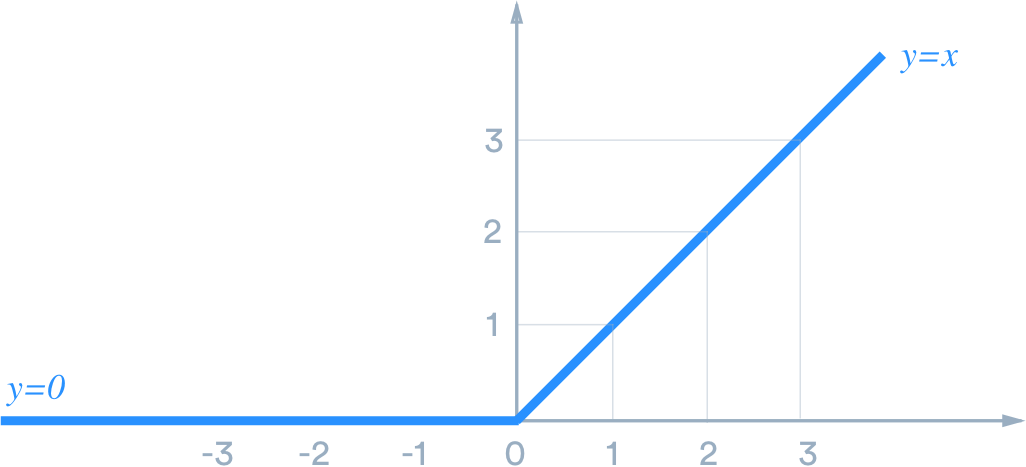
\includegraphics[width=10cm]{relu}

\subsection{Sigmoid Activation Function}
The sigmoid activation function is a non-linear activation function that looks like an S-shape. Any small changes in the incoming $X$ value (the calculated sum) will cause the $Y$ value (the output) to change significantly. The range of the function is $(0,1)$. That means the range is bounded, which means it does not blow up. The disadvantage of the sigmoid activation function are the vanishing gradients \ref{vgp}.\\

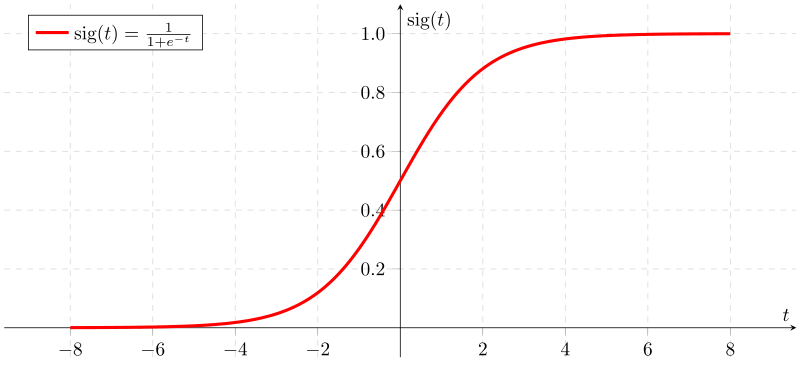
\includegraphics[width=10cm]{sigmoid_function}

\pagebreak

\subsection{Tanh Activation Function}
The tanh activation function resembles the sigmoid function. The difference is that the range of tanh activation function is $(-1,1)$. Another difference is that the gradients are stronger for tanh than sigmoid. That means the derivatives are steeper. One benefit tanh has over sigmoid, is that it  avoids biases in the gradients \cite{Tan_h}.\\\\

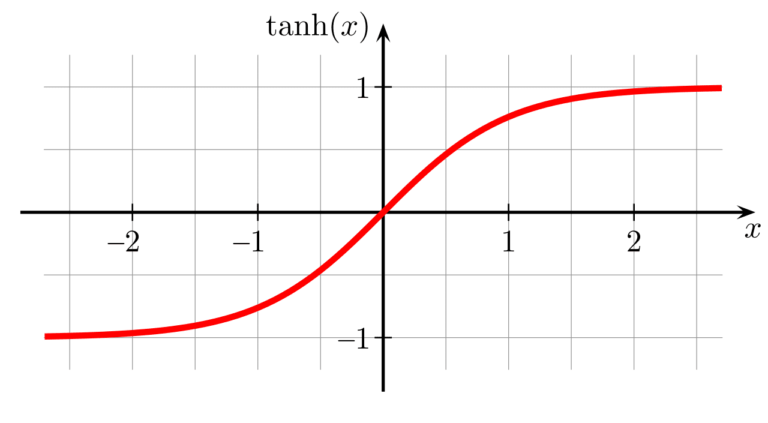
\includegraphics[width=10cm]{tanh_function}

\section{Recurrent Neural Networks}
Recurrent neural networks (RNN), are a type of neural network that uses the output from the previous step and feeds this output as input in the current step. Whereas in traditional neural networks, the network assumes that the inputs and outputs are independent of each other. The cost function or error in RNN can be calculated at any time $t$. At any time $t$, the current input is a combination of inputs $x_t$ and $x_{t-1}$. This makes the neural network recurrent, it has feedback loops at each iteration of the hidden layer. Recurrent neural networks are used for Sequence Modeling. Sequence Modeling is the task to predict future outcomes. \\\\
However, there are some drawbacks to RNN. The first drawback is when the sequence is done in order, there is a limit in how much training can be parallelized. The second drawback is that the farther away the relevant points in the sequence are from one another, the harder and slower it is to make connections between them. This drawback is caused by the vanishing gradient problem.\\

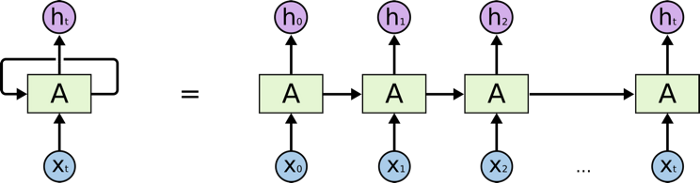
\includegraphics[width=12cm]{RNN}

\subsection{Vanishing Gradient problem}\label{vgp}
The vanishing gradient problem can be encountered when gradient-based learning methods and backpropagation are used. Adding more layers using non-linear activation functions to the neural network causes the gradients of these loss functions to approach zero. The gradient will be vanishingly small, which in turn prevents the current weight from changing its value. This can lead to the neural network to stop training further. As mentioned before, an activation function like the sigmoid function, squishes a large input space into a value between 0 and 1. The effect of this is that a large change in input would cause a small change in the output. The derivative therefore becomes miniscule. The derivative approaches zero, which causes the gradient of this layer in the network to vanish. \\\\
One of the network that suffers from the vanishing gradient problem is a basic recurrent neural network. When the feedback loops occur and the gradient gets lower, it becomes harder for the network to update its weights. The weights of the initial value will not change effectively through the training process, which can lead to inaccuracy in the network. \\\\
The solution to the vanishing gradient problem is to use activation functions for the network that are resilient to this problem, such as ReLu. This is because ReLU does not cause a small derivative. Another solution is to use resilient neural networks, such as residual networks \cite{DBLP:journals/corr/HeZRS15}. There are also specialized RNNs that are more resistant to this problem. One of these specialized networks is the long short-term memory (LSTM) network. 

\subsection{LSTM}
Long short-term memory (LSTM) is a specialized RNN that is capable of learning in long-term dependencies. It is designed to remember information for long periods of time. It does this by adding a forget mechanism. The hidden layer in LSTM is a gated cell. It consists of four layers that interact with each other to produce the output of that cell to pass on to the next hidden layer. LSTM consists of three logistic sigmoid gates and one tanh layer, compared to traditional RNNs that use only a single layer of tanh. These gates are used in order to limit information or pass information through the cell. The inputs of LSTM go through the input, forget and output gate. The forget gate decides to remember or to skip inputs from the previous hidden states. The mechanism of the forget gate mostly solves the vanishing gradient problem. The input gate decides what new information has to be added to the cell. Finally the output gate decides which new or old information has to be passed to the next hidden layer by using the memory state that is updated by the input and forget gate. \\\\

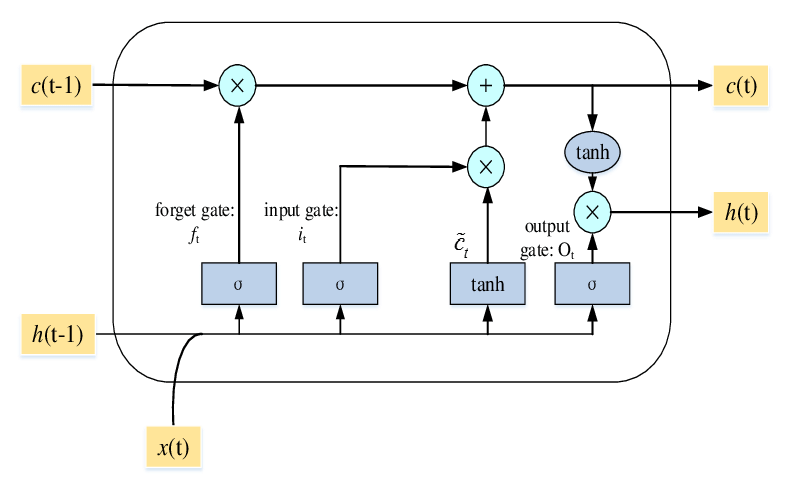
\includegraphics[width=12cm]{LSTM}
\\ While LSTM overcomes the vanishing gradients in the network, it inherits some problems of RNNs, such as: no parallelization, as there is a sequential path for the data in the network. While LSTMs have mitigated the vanishing gradient problem, it could not completely get rid of the problem. The data in LSTM has to move from cell to cell in a sequential manner, same as in traditional RNN. This problem inherently lies in the recursion of RNNs. RNNs can be slow to train, but LSTMs are even slower to train, because they are more complex than traditional RNNs. 

\section{Transformers}
A transformer is a new network architecture in which the input sequence can be passed in parallel, which can increase the speed drastically. The transformer is first introduced by Vaswani et al. in their paper \textit{”Attention Is All You Need”} \cite{Transformers}. The transformer model is based solely on the attention mechanism. Attention is a mechanism that figures out for each token, how relevant all the other tokens are in a sequence. Attention learns to weigh the relationship of each token in the input sequence to other tokens in the output sequence. The core idea is that the transformer model uses only the part of the input where the most relevant information is concentrated instead of the entire sequence. The same as a neural network is considered to mimic a human brain, the attention mechanism also tries to implement the action of selectively concentrating on relevant things, while ignoring other not relevant inputs in the neural network. Self attention is similar to attention, but it allows the inputs not to only interact with the outputs, but with other inputs as well.  The transformer model that Vaswani et al. proposes in their paper uses multi-headed attention layers. In multi-headed attention, each head in the layer learns attention relationships independently. Attention is constructed as a combination of three matrices, where every value in those matrices are learned.\\
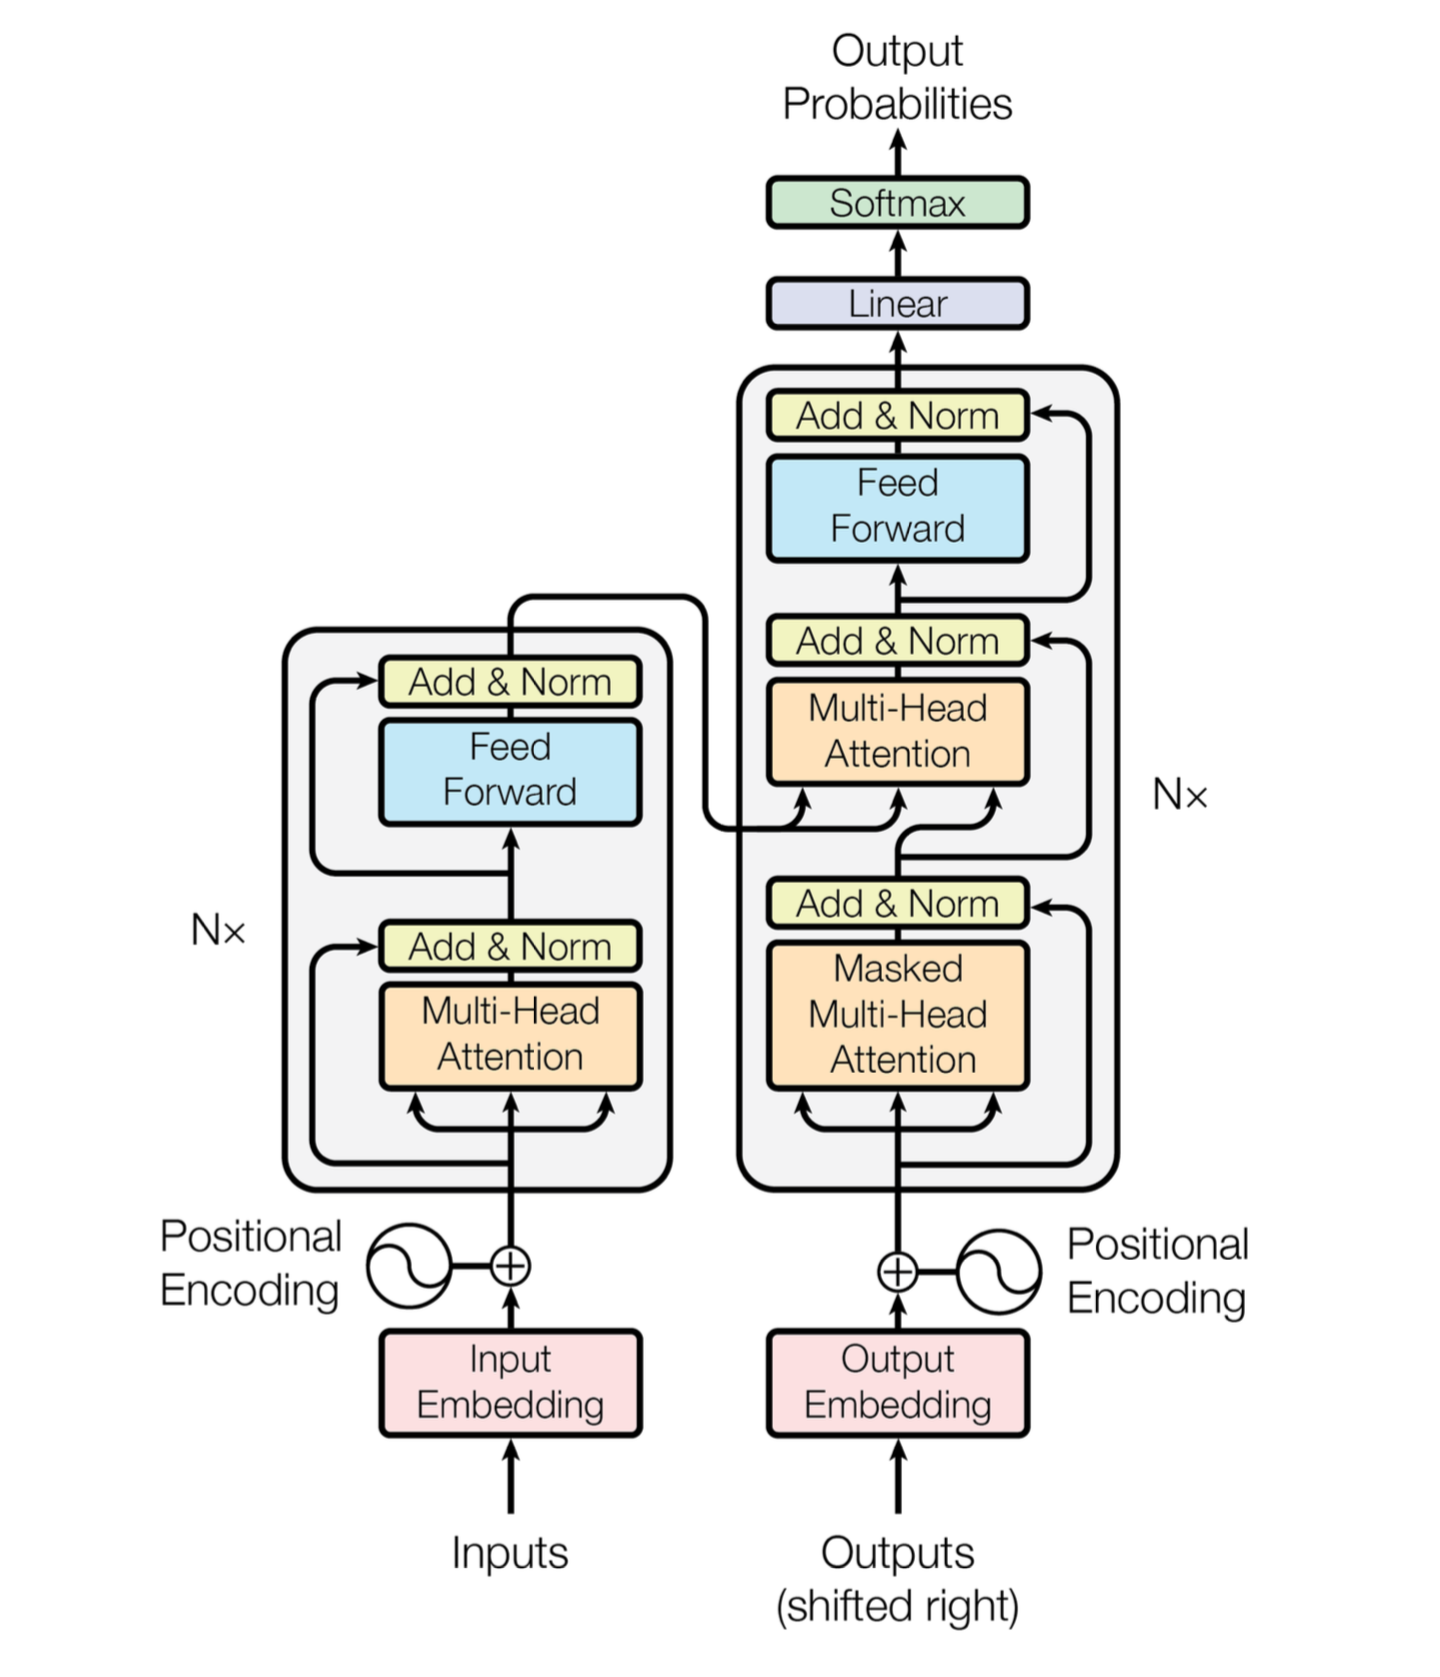
\includegraphics[width=12cm]{transformer}
The transformer architecture that is proposed in the paper, uses a sequence to sequence model \cite{sts}, that consists of an encoder and a decoder. Before the inputs go into the encoder, the input has to be embedded. Input embedding maps every word to a point in space where similar words or meanings are physically closer to each other in that space. This space is called the embedding space. The embedding space maps a word to a vector. In a sentence the same words can have different meanings. That is why transformer models have positional encoders. These encoders are vectors that give context based on the position of a word in a sentence. Adding positional encodings to a transformer model will result in embeddings of words with context information. The resulting input embedding with context information then goes into the encoder. This encoder contains a stack of multi-headed attention and a feed-forward neural network \cite{ffn}. These feed-forward neural networks are used to transform the attention vectors to make it digestible for the next encoder or decoder block. The decoder is similar to the encoder, only it has an additional multi-head attention block. Transformers are used for sequence to sequence tasks like NLP or machine translation. It is also used as autoencoding language modeling, such as masked language modelling. One of the models that is trained on masked language modeling, created by Google, is called BERT. 

\subsection{BERT}
BERT (Bidirectional Encoder Representations from Transformers) is a large transformer masked language model. It is mostly used for pre-training natural language processing (NLP). The main innovation of this technique is applying bidirectional training on a Transformer model. In contrast, other efforts looked at it in a single direction, from left to right or right to left.\\\\
BERT uses the encoder mechanism to generate a language model. Bert's encoder reads the entire sequence of words at once.  Therefore, it ensures that the model learns the context of a word from all of its surroundings, making it bidirectional. BERT are pretrained on two tasks: language modelling (LM) and next sequence prediction (NSP). It uses Masked LM (MLM) for pretraining language modelling. This is done by replacing 15\% of any sequence with a [MASK] token. The model tries to predict the original value of the masked words, using the context provided by the other non-masked words in a sequence. Masked language models are a type of contextual word embedding models. Contextual word embedding gives a model different representation for different sentences. 
\pagebreak
\\The next task of the training process, BERT uses next sentence prediction to better understand the relationship between two sentences. While the model is training it receives sentences as input pairs and it learns to predict if the second sentence in the input pair is also the next sentence that was in the original document. BERT separates sentences with a special [SEP] token. Then the model is fed with two input sentences at a time. During training, 50\% of the time the second sentence is the subsequent sentence in the original document, while in the other 50\% of the time it is a random sentence from the full corpus. The assumption being that the random sentence will be disconnected from the first sentence.\\\\
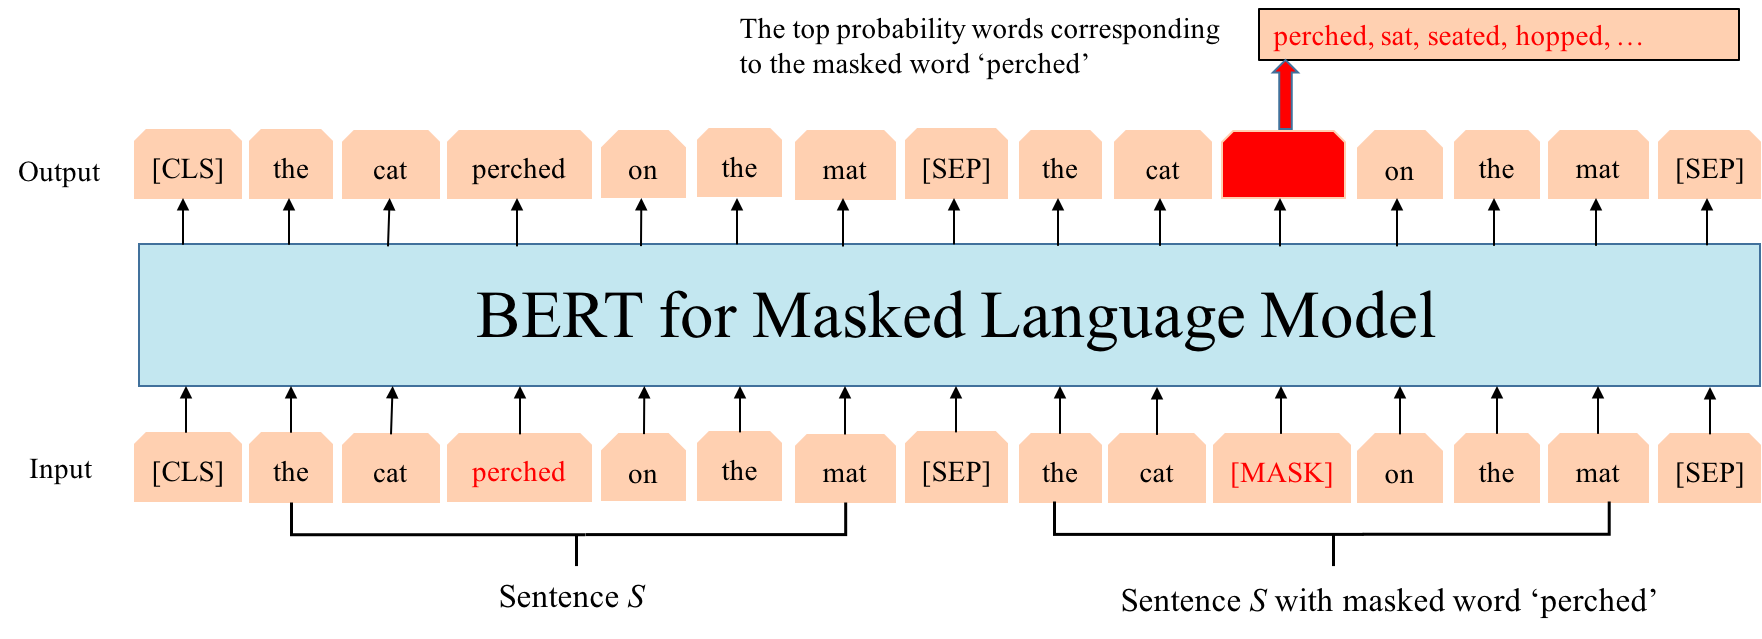
\includegraphics[width=13cm]{BERT}\\\\
All together the input in BERT is processed in these six steps: 
\begin{enumerate}
    \item Each sentence sequence is separated by a [SEP] token. It is placed at the end of each sentence.
    \item Every sentence will replace 15\% of its words with a [MASK] token.
    \item At the beginning of the first sentence a special [CLS] token will be inserted.
    \item Every other word in a sentence is transformed into an embedded token.
    \item A sentence embedding is added to each token. They are similar in concept as token embeddings, but these embeddings are used to indicate if sentence A or sentence B is added to each token.
    \item At last a positional embedding gets added to every token to indicate their position in the sequence.
\end{enumerate}
